% HEADER BEGINS
\documentclass[10pt]{article}
%% Packages
\input{settings/packages}
\usepackage{graphicx}
\usepackage{float}
\usepackage{enumitem}
\usepackage{fancyhdr}
\usepackage{rotating}
%% Page Settings
\input{settings/page}
%% Own Commands
\pagestyle{fancy}
\fancyhf{}
\fancyhead[CE,CO]{Early Detection of MCI that progresses to dementia - An Interdisciplinary Approach}
\fancyfoot[LE,RO]{\thepage}

\renewcommand{\headrulewidth}{2pt}
\renewcommand{\footrulewidth}{1pt}
\input{settings/macros}
\title{Qualifying Report}
\date{2019-01-31}
\author{Jomar Alcantara}
% HEADER ENDS
% DOCUMENT BEGINS
\begin{document}
\section{Abstract}
\section{Background}
Dementia has been identified as one of the fastest growing difficulties facing the world today. A recent report suggests that in 2015 there were 46 million people with a diagnosis of dementia and that number is expected to hit 131.5 million by 2050 \cite{Prince2015}. The report also states that the worldwide cost of dementia in 2018 is estimated to be in the region of one trillion US dollars.
\par
In 2009, the Department of Health designed it's National Dementia strategy and as part of this made early diagnosis and support one of it's key priorities \cite{England2009}. A lot of work has gone into trying to find ways of improving the early diagnosis of Alzheimer's Disease (AD) and Mild Cognitive Impairment (MCI) with research focused on two areas - identifying biological markers and analyzing the cognitive decline of those who are suspected to have the disease \cite{Taler2008}. As described above, the numbers of those suffering from AD and MCI are going to increase as the population ages \cite{Prince2015} and thus it is important that we utilize technology wherever possible to aid clinicians in the detection of MCI and AD. At the present time diagnosis is typically conducted at memory clinics by trained clinicians \cite{Boschi2017}. I theorize that we may be able to enable an earlier diagnosis of those with MCI and AD using samples of spontaneous speech, natural language processing (NLP) and machine learning (ML).
\par
There is a large body of research that looks at the decline in language of those with MCI and AD \cite{Taler2008, Boschi2017}. However there is conflicting evidence in these studies about which declining language factors are associated with MCI and AD \cite{Taler2008, Boschi2017}. Research therefore should look at these features in more detail and a clarification of this currently disorganised picture should go some way to helping researchers further understand the disease and it's progression. There is some evidence to support this, Berisha et al \cite{Berisha2015}, has shown through a longitudinal language analysis of spontaneous speech that there are marked differences in different parts of speech in this process between those who would go on to have a diagnosis of AD and a healthy control. 
\par
The potential impact of this research in this area is immense. Research has shown that early diagnosis of people with AD or MCI improves sufferers quality of life and can, in some cases, slow the progress of the disease. Early diagnosis can increase the number of research opportunities for understanding the early stages of dementia and how the disease progresses so that more research can be conducted which may, in the future, lead to new treatments and other interventions.


There has been a significant research in the area of language deterioration as a means of detecting Alzheimer's Disease. This usually takes the form analysis of speech recorded as part of a cognitive assessment such as the Picture Description Task \cite{Orimaye2014,Fraser2015}. Given that language samples are relatively easy to collect, research has moved towards analysis of spontaneous speech. An good example of this type of research is the study conducted by Berisha and Liss which looked at the differences in language use between two US presidents, Ronald Reagan (who would go on to receive a diagnosis of Dementia) and George H.W. Bush who acted as a matched control based on Age \cite{Berisha2015}. They found several differences in language use which they felt acted as indicators of Reagan's difficulties with language due to dementia. These significant differences were in the number of unique words used per speech, the use of non-specific nouns and fillers and low-imageability verbs \cite{Berisha2015}. 
\par   
This study replicates work done by Berisha and Liss and extends this by adding Donald Trump as an alternative, more appropriate comparison to Ronald Reagan as he is much closer in age than George H.W. Bush. This experiment will look at the features originally identified by Berisha and Liss, as well as any others that have potential as discussed in the literature review above. 
\section{Methodology}
I took 46 transcripts of Ronald Reagan’s (RR) press conferences from 1981 to 1988 and compared them with 134 press conferences by George H. W. Bush (GHWB) and 29 press conferences conducted by Donald J. Trump (DJT).  I analyzed transcripts for lexical features shown to change longitudinally with dementia  (for a comprehensive review of these, see the literature review above). For this collection of documents, I generated a number of features which looked at a number of different aspects of each document. These features encompassed, word level, sentence level and document level features and included a number of features contained in the study by Berisha and Liss with the aim of replicating and extending on their findings. These findings were. number of unique words, non-specific nouns and fillers and low imageability (LI) verbs. Imageability is characterized, according to Berisha and Liss, as the ease with which a term gives rise to a sensory .mental image. I compared the trends described in the transcripts of RR and GHWB, but also included DJT. Berisha and Liss originally made the comparison as it GHWB (GHWB - age at the start of presidency - 64 years, 222 days) was the closest match to RR in terms of age (RR  - age at the start of presidency, 69 yeaars and 349 days). However, with the inauguration of Trump, he now is the closest comparible president in terms of age (DJT - age at the start of presidency - 70 years, 220 days). It would be interesting to look at a comparison of RR and DJT to see whether the comparisons made by Berisha and Liss hold true with this more appropriate match (in terms of age). DJT as with GHWB has no known diagnosis of AD. I used the press conference transcripts in the American Presidency Project (APP) archive as a data source for this project. The APP is a comprehensive and organized searchable database of presidential documents, including transcripts of speeches, transcripts of news conferences, and other public documents.
\subsection{Pre-processing}
To generate the files necessary for analysis, I downloaded each transcript and performed the following changes. I omitted the prepared statement by the president and any speech by other individuals. I started each transcript at the beginning of the first answer to a question. I filtered any annotations that were added to the transcript, including any references or clarifications, and any laughter. It's worth noting that there appears to be a difference in how 'hesitations' were marked down between each president, for RR hesitations were marked by a single hyphen whereas for GHWB hesitations are marked by a double hyphen. In order to maintain consistency when parsing through the documents, I have changed both types of hesitation to be marked by a single hyphen. I also omitted one word sentences as this data would, from a theoretical perspective, not be relevant for language analysis. I did not control for the length of the document, but generated features which would normalise by the length of the document. I therefore was able to include all press conferences by both Ronald Reagan and George H.W. Bush where there was a question and answer session conducted at least in part by the sitting president (2 press conferences of GHWB were ommited due to a lack of a question and answer session).
\subsection{Feature Selection}
We calculated the following features for each transcript in turn using the NLTK (see section 2 for a description) \cite{Bird2009} and Python. 
\par 
\subsubsection{Measures of lexical variation}
We constructed two features of lexical variation. Firstly we looked at the number of unique words. To do this we were able to split each transcript into individual words and changed them to lowercase using NLTK and were then count the number of unique words that appeared in each transcript. We also used the TTR formula (see section 2 for a description) for a feature that measures lexical diversity independent of sample size \cite{Richards1987}. 
\subsubsection{Fillers, Non-Specific Nouns and LI Verbs}
For these features, we counted the number of occurrences for different categories (see table for list of categories tracked and the words counted). The features were used by Berisha and Liss in their research \cite{Berisha2015} and were taken from work done by Bird et al \cite{Bird2000}. 

\begin{table}[H]
	\begin{center}
	\begin{tabular}{ | p{3cm} | p{6cm} |}
		\hline
		Category & Words \\ \hline
		Fillers & \textit{"well", "so", "basically", "actually", "literally", "um", "ah"} \\ \hline
		Non Specific Nouns & \textit{"something", "anything", "thing", "everything"} \\ \hline
		LI Verbs & \textit{"be", "come", "do", "get", "give", go", "know", "look", "make", "see", "tell", "think", "want"} \\ \hline
	\end{tabular}
	\caption{\label{tab:table-name}Categories and Words Counted}
	\end{center} 
\end{table}

\subsubsection{Usage of parts of speech}
This section involves using a Part of Speech tagger (PoS) which analyses a sentence and assigns a 'tag' to each word based on the function the word has in a sentence. At a basic level this can be divided into the eight defined parts of speech: 'nouns', 'pronouns', verbs', 'adjectives', 'adverbs', 'conjunctions', 'prepositions' and 'interjections' but can be further subcategorised. We used the PoS tagger built into NLTK to tag each transcript in turn and used these the counts from each of these eight categories in our analysis. In addition to frequency counts we also normalised these features by dividing the frequency count by the number of words in the document to take into account transcript length.

\section{Results}
One of the most important thing to note is the wide variety of samples between the three presidents and also the varying timescales. RR participated in 46 press conferences over eight years (an average of 5.75 a year) which is the fewest number of press conferences given by an American president during their term of office. GHWB participated in 136 press conferences over four years (an average of  34 a year) and DJT participated in 29 press conferences to date (an average of 19.3 per year). Equally, there are variances in the average number of words. RR produced an average of 3424 words per conference compared to 2608 by GHWB (unpaired t = 4.434, p\textless 0.001) and DJT at 1849 words (unpaired t = 6.524, p\textless 0.001).
\begin{table}[H]
	\begin{center}
	\begin{tabular}{ | p{3cm} | p{1.5cm} | p{1.5cm} | p{1.5cm} |}
		\hline
		& RR & GHWB & DJT \\ \hline
		Total Words & 3423.91 (416.42) & 2607.72 (1210.38) & 1848.65 (1549.38) \\ \hline
		Unique Words & 894.13 (85.15) & 667.76 (218.67) & 481.82 (221.29) \\ \hline
		Non Specific Nouns & 12.72 (4.63) & 6.78 (4.32) & 7.41 (8.75) \\ \hline
		LI Verbs & 124.22 (17.89)& 103.45 (51.87) & 84.48 (75.78) \\ \hline
	\end{tabular}
	\caption{\label{tab:table-name}Means and Standard Deviations of important features}
	\end{center} 
\end{table}

In terms of unique words, we found that RR used significantly more unique words, non-specific nouns and low imageability verbs than GHWB and DJT (see Table 3.3). Some of these differences are due to the length of the sample, particularly in the case of DJT where his average sample is almost half the sample of RR. It could also be said that this could be down to differences in linguistic abilities or speaking style \cite{Berisha2015, Le2011}. However, we can certainly see that as controls GWHB and DJT are comparative in relation to non-specific nouns and LI verbs. 

\begin{table}[H]
	\begin{center}
	\begin{tabular}{ | p{3cm} | p{1.5cm} | p{1.5cm} | p{1.5cm} |}
		\hline
		& RR v GHWB & RR v DJT & GHWB v DJT \\ \hline
		Total Words & \textbf{4.434***} & \textbf{6.524***} & \textbf{2.899**} \\ \hline
		Unique Words & \textbf{6.832***} & \textbf{11.403***} & \textbf{4.137***} \\ \hline
		Non Specific Nouns & \textbf{7.877***} & \textbf{3.426**} & -0.574 \\ \hline
		LI Verbs & \textbf{2.656**} & \textbf{3.420***} & 1.628 \\ \hline
		\multicolumn{4}{@{}p{1.5in}}{\footnotesize * denotes p\textless 0.05} \\
		\multicolumn{4}{@{}p{1.5in}}{\footnotesize ** denotes p\textless 0.01} \\
		\multicolumn{4}{@{}p{1.5in}}{\footnotesize *** denotes p\textless 0.001} \\
	\end{tabular}
	\caption{\label{tab:table-name}RR T-tests vs GWB and DJT}
	\end{center} 
\end{table}

We then looked at the data from a longitudinal perspective as we are interested seeing whether we can track various language variables and their progress over time. We ran a number of Pearsons correlations with transcript index number as a time reference and the dependant variables (Table 3.4).  For our controls, we found them to be stable for the most part with the main highlights being a decrease in Adverb usage for DJT (R=-0.36, p=0.049) and a steady but not severe decline in a number of variables for GWHB, namely total word count, unique words, low imageability words and verb usage.
\par 
For RR, his decline is more marked and more widespread through his language use. We noticed an significant increase in adverb (R=0.41, p=0.004) and pronoun usage (R=0.65, p\textless0.001), as well as a slight usage increase in Non-specific nouns(R=0.30, p=0.03). There was a highly significant decrease in number of unique words (R=-0.56, p\textless0.001) and noun usage (R=-0.70, p\textless0.001). Also very significant decrease in adjective usage (R=-0.40, p=0.005) and a significant decrease in total word count (R=-0.31, p=0.03). 

\begin{table}[H]
	\begin{center}
	\begin{tabular}{ | l | p{1.5cm} | p{1.5cm} | p{1.5cm} |}
		\hline
		& RR & GHWB & DJT \\ \hline
		Word Count & \textbf{-0.31*} & \textbf{-0.21*} & 0.08 \\ \hline 
		Unique Words & \textbf{-0.56***} & \textbf{-0.25**} & 0.16 \\ \hline
		Non Specific Nouns & \textbf{0.30*} & -0.08 & -0.03 \\ \hline
		LI Verbs & -0.19 & \textbf{-0.20**} & 0.02 \\ \hline
		Nouns Normalised & \textbf{-0.70***} & -0.03 & 0.14 \\ \hline
		Verbs Normalised & \textbf{0.36**} & \textbf{0.24***} & -0.03 \\ \hline
		Adjectives Normalised & \textbf{-0.40**} & 0.08 & -0.34 \\ \hline
		Adverbs Normalised & \textbf{0.41***} & 0.02 & \textbf{-0.36*} \\ \hline
		Pronouns Normalised & \textbf{0.65***} & 0.13 & 0.07 \\ \hline
		\multicolumn{4}{@{}p{1.5in}}{\footnotesize * denotes p\textless 0.05} \\
    	\multicolumn{4}{@{}p{1.5in}}{\footnotesize ** denotes p\textless 0.01} \\
    	\multicolumn{4}{@{}p{1.5in}}{\footnotesize *** denotes p\textless 0.001} \\
	\end{tabular}
	\caption{\label{tab:table-name}Pearson Correlations for Features}
	\end{center} 
\end{table}

\section{Discussion}
President Reagan received his diagnosis of AD in August 1994 but using transcripts of speeches he made in his two terms as President (January 1981 - January 1989) we have be able to identify certain changes in his use of language that we might ascribe to the onset of MCI and early AD. Despite differences in our methodology, our research supports the findings of Berisha and Liss in that we both find a significant decrease in unique words over time and an increase in non-specifc noun usage. Compared to our controls (GWHB andDJT), we find some slight trends with GWHB but no such trends with DJT in his speech albeit his samples of speech span a shorter amount of time.
\begin{figure}[H]
	\centering
	\begin{minipage}[b]{0.4\textwidth}
		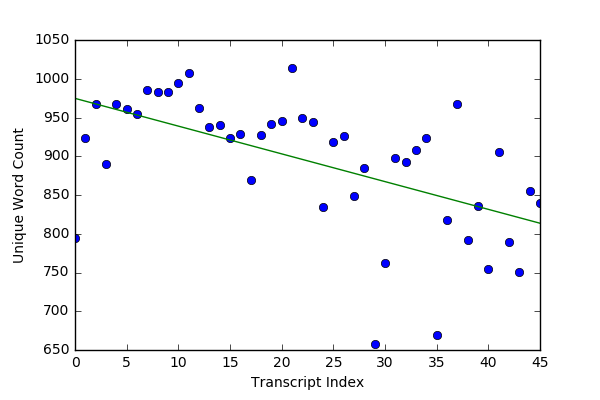
\includegraphics[width=190px, height=140px]{images/RRUniqueWords.png}
		\caption{Ronald Reagan - Unique Words over time}
	\end{minipage}
	\hfill
	\begin{minipage}[b]{0.4\textwidth}
		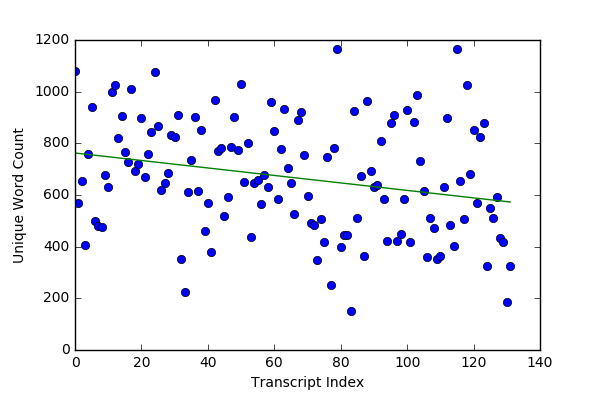
\includegraphics[width=190px, height=140px]{images/GWHBUniqueWords.png}
		\caption{George H.W. Bush - Unique Words over time}
	\end{minipage}
\end{figure}

\begin{figure}[H]
	\centering
	\begin{minipage}[b]{0.4\textwidth}
		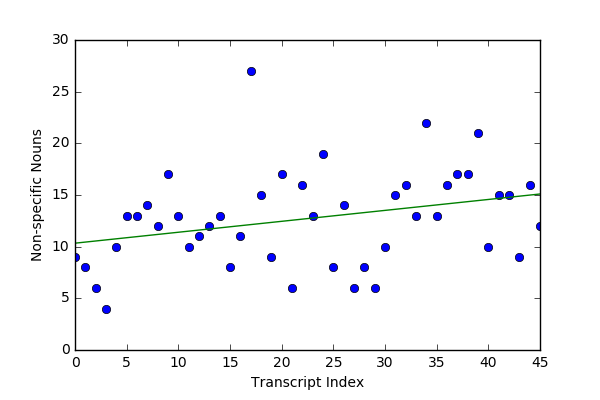
\includegraphics[width=190px, height=140px]{images/RRNSNouns.png}
		\caption{Ronald Reagan - Non-specifc Nouns over time}
	\end{minipage}
	\hfill
	\begin{minipage}[b]{0.4\textwidth}
		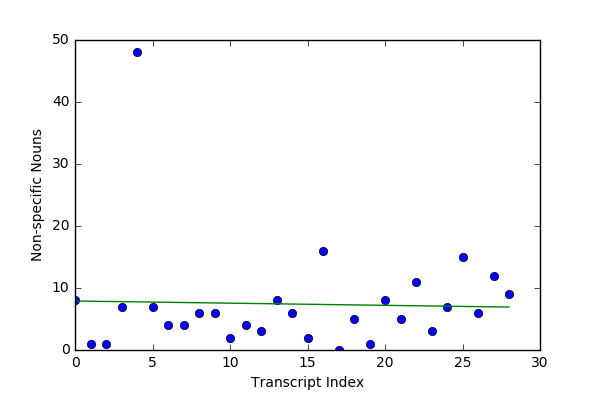
\includegraphics[width=190px, height=140px]{images/DJTNSNouns.png}
		\caption{Donald J. Trump - Non-specific Nouns over time}
	\end{minipage}
\end{figure}

A criticism of Berisha and Liss's work is the problems they had with normalising the transcripts in terms of length. This was also a problem in the work of Garrard et al \cite{Garrard2005, Le2011}. Whilst it is important to control for outliers, there are other ways in which we can control for length of sample.  
\par 
Interestingly, when we normalised the various types of words used by the presidents we found some interesting patterns that further differentiated RR from the controls. Whilst Non-specific nouns increased over time, we found that noun usage in general significantly decreased and pronouns increased similarly significantly. The increase in pronoun for those with early AD has been identified in literature, although there are only a few studies that explore this \cite{Almor1999, Wendelstein2015}. Wendlestein et al propose that the increased used of pronouns is an expression of an impaired ability to adapt language to the listener's needs \cite{Wendelstein2015}. Almor et al attributed this reliance on pronouns due to a impaired working memory \cite{Almor1999}.
\par 
The decrease in overall noun usage has also been identified as a feature. Jarrold et al found that AD patients would use more pronouns, verbs and fewer nouns than controls \cite{Jarrold2014}. Wendlestein in their investigations into noun usage found that decreased later on in AD progression and was unaffected in the pre-clinical stages of AD \cite{Wendelstein2014}. Our results are supported by existing literature and this potentially means that language analysis in the way we have structured it may have diagnostic or prognostic properties.

\begin{figure}[H]
	\centering
	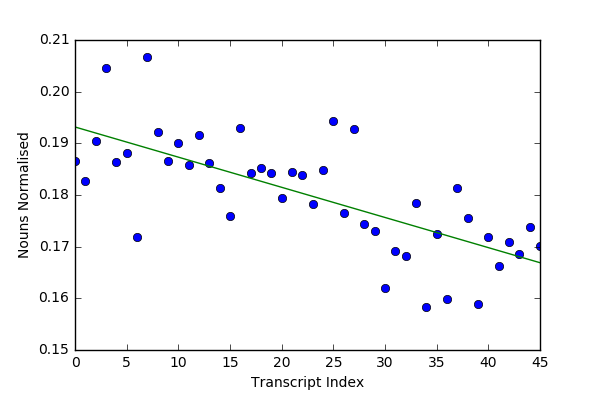
\includegraphics[width=240px, height=150px]{images/RRNounsNormalised.png}
	\caption{Ronald Reagan - Nouns Normalised over time}
\end{figure}

\begin{figure}[H]
	\centering
	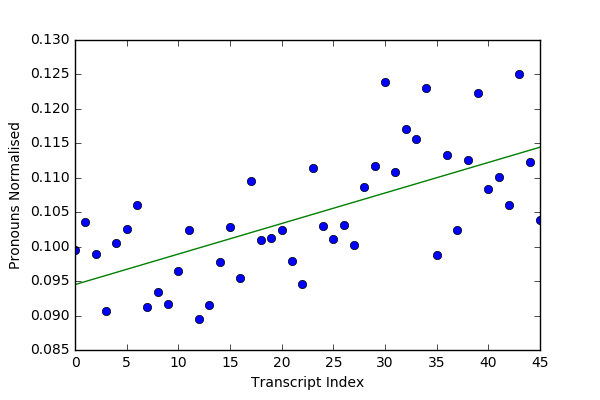
\includegraphics[width=240px, height=150px]{images/RRPronouns.png}
	\caption{Ronald Reagan - Pronouns Normalised over time}
\end{figure}
 
There are limitations of this research. Whilst in terms of age, DJT is certainly more suitable as a control to match with RR, in some ways they held very different styles of press conferences in that RR preferred to do solo press conferences and DJT has shown a preference for doing joint press conferences which have an impact on the amount of language produced. This artifact of the data is in itself notable as it illustrates the problems we may have with smaller amounts of speech. Also, the problem of finding an appropriate control is a common one in this domain. Given that those with MCI and early dementia have such variable presentations, it might prove of limited value in matched pairs design. 
\par 
With further work, it is not feasible to the vast array of samples over a timeframe, as we have had with the president corpus and so it would be worth exploring how the quality of these predictions might lessen when faced with considerably fewer samples and over a smaller time period. It would also be worth extending this research further to encompass more of the linguistic features Fraser used in her work \cite{Fraser2015} to see if there are any further insights to be gained. In addition, this replication and extension has demonstrated the potential utility of using longitudinal data as a means of comparing language use of a person at two or more time periods and using this information as a diagnostic aid for MCI and therefore more work would be helpful from a longitudinal perspective to see if this approach may be valid in moving towards a solution for this particular problem. 
\par 
The results of this work show that we can track a person's use of language through time in a number of ways, and it is possible for an individual to be his or her own control. This is important as it means the heterogenous nature of the MCI population does not impact results as much as if we were comparing those with MCI to controls. Equally, it would be helpful to have controls to ascertain what would be usual to expect in the decline of language in a healthy older adult. 



\bibliographystyle{unsrt}
\bibliography{QualifyingReport}

\end{document}
%DOCUMENT ENDS